\chapter{Preliminary study}
\lhead{\textit{Chapitre \thechapter}}
\rhead{\textit{Premier chapitre}}

\section{Introduction}
Lorem ipsum dolor sit amet, consectetur adipisicing elit, sed do eiusmod
tempor incididunt ut labore et dolore magna aliqua. Ut enim ad minim veniam


\section{General Definitions}
\subsection{Website}
A website is a collection of publicly accessible, interlinked Web pages that share 
a single domain name. Websites can be created and maintained by an individual, group, 
business or organization to serve a variety of purposes.\cite{Techopedia2011-zo}

\subsection{Responsive Web Design}
Responsive web design (RWD) is a web development approach that creates dynamic 
changes to the appearance of a website, depending on the screen size and orientation of 
the device being used to view it. RWD is one approach to the problem of designing for 
the multitude of devices available to customers, ranging from tiny phones to huge desktop monitors.\cite{noauthor_undated-an}

\subsection{Interactive Course}
The term "Interactive Course" (IC) typically describes material of an educational nature 
delivered in a format which allows the user to directly impact the materials content, pace, and out-come.
An example of such material would be a computer based presentation requiring a user to select the correct 
answer to a give question before proceeding to the next topic.
These types of courses are almost always computer based and most likely to be delivered to the user thru the internet. 
Due to their convenient delivery, availability and almost endless subject matter, 
interactive courses have become a major tool for those seeking to provide as well as those seeking to obtain education, 
training or certification in a given area of study.\\
With growing access and availability to computers and the internet, many schools, universities, 
businesses and government agencies are turning to IC's to train and educate their students and staff.\cite{noauthor_undated-dt}

\subsection{Computer Architecture}
\subsubsection{In general}
Computer architecture is a science or a set of rules stating how computer software and hardware are 
joined together and interact to make a computer work. It not only determines how the computer works 
but also of which technologies the computer is capable.\cite{Pam2018-so}
\subsubsection{In our case}
Computer architecture or better known as "Structure Machine"(STRM) is a course for first-year 
students in the Math and Computer Science department (MI) 
of the university bouira AMO. and also in all the MI departments in Algeria universities.\\ \\
\indent Computer architecture (STRM) has a coefficient of 3 and a credit of 5, which makes it one of the more fundamental courses.

\section{Study of the existing}
We did go over the definition of computer architecture in a general sense and in our context of study(STRM),
so in this part we will go more in-depth about the structure of the computer architecture(STRM) course (see Figure~\ref{fig:STRM}), and which resources we will be basing our own study of the course from.

\subsection{Structure of the computer architecture course}

\begin{figure} [h!]%[htbp]
 	\vspace*{13pt}
 	\subfloat{\label{}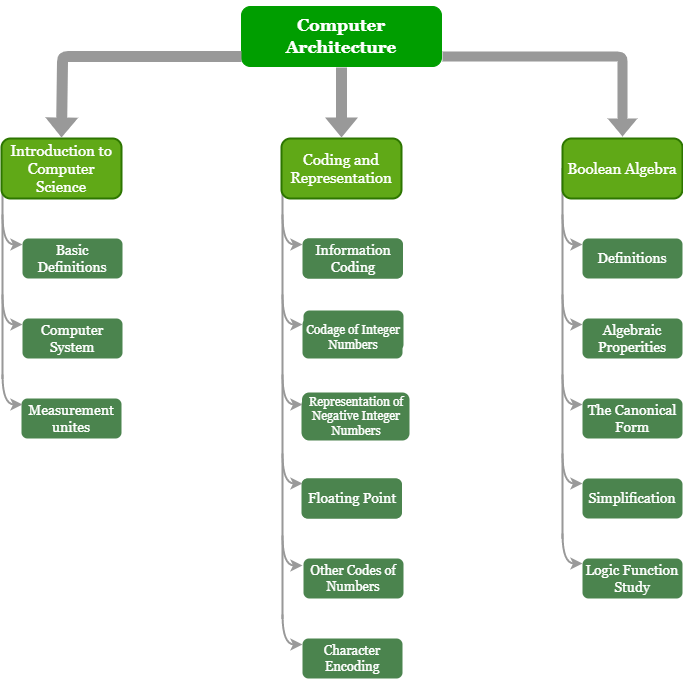
\includegraphics[scale=0.63]{img/STRM.png}} 
 	\vspace*{13pt}               
 	\caption{Structure of STRM} 
 	\label{fig:STRM}
 \end{figure} 

 \subsection{Computer architecture course}
 there exists some books that cover the course of computer architecture, and based on our experience as a students of the MI department that has already studied this course 
 we would like to mention the following :
 \subsubsection{Digital Design and Computer Architecture :}
This book by David Harris and Sarah Harris is designed for courses that combine digital logic design with computer organization/architecture or that teach these subjects
as a two-course sequence. Digital Design and Computer Architecture begins with a modern approach by rigorously covering the fundamentals
of digital logic design and then introducing Hardware Description Languages (HDLs). By the end of Digital Design and Computer Architecture,
readers will be able to build their own microprocessor and will have a top-to-bottom understanding of how it works--even if they have no formal background
in design or architecture beyond an introductory class. \cite{harris2010digital}

\subsubsection{STRM 1 Book :}
This book by Dr. Taha Zerrouki is a lessons and solved exercises focus, intended for first-year students of mathematics and Computer Science department (MI) in 
Algerian universities.\cite{STRM-1-Book-Taha-Zerrouki}\\
It contains in this part the lessons of the first semester:
\begin{itemize}
	\item Interoduction to computer science.
	\item Coding and representation of information.
	\item Boolean Algebra.
\end{itemize}
The book contains a large number of exercises divided according to chapters, a large part of it is solved, as well as a special section for continuous assessment examinations with
Correction, and another section for exams.
This book comes as a result of the experience that Dr Taha gained in teaching at the University of Bouira for many years in the Department of Computer Science.
The book is also bilingual, with lessons in French and translated into Arabic, in order to help new students who suffer from a language barrier in their college start.
\footnote{We will be focusing our study of the course on the STRM 1 book \cite{STRM-1-Book-Taha-Zerrouki}}


 \section{Analysis of existing applications}
 In this presentation ,we will talk about applications, books and similar resources about computer science, 
 where we will discuss its most important characteristics and advantages.
 There are many applications similar to our topic, but they do not contain all computer science topics.
 As for books and websites, there are many that include all computer science lessons, but they do not 
 contain the practical aspect that we will work on.
 

 \subsection{STRM Tests}
 Dr.Taha built this app to generate and create random tests for Stucture Machine 1- first Year MI, Mathematiques and Informatiques
  in Algerian universities.\cite{STRM-Tests}
 
 What this app contains:
 • Generate checks and questions with solutions
 
 • Supports the following classes:
 
 - Enumeration systems.
 - Representation of natural and real numbers and letters.
 - Encoding information.
 - Boolean algebra.
 
 • Generate answers:
 
 - Possibility to draw a logical function diagram.
 - Generate Karnoff tables.
 - Generating graphic solutions to Karnoff's table.
 
 • Generate duplicate forms of questions for easier typing.
 
 • Random generation of questions.
 
 \subsection{Computer Architecture from saylor academy}
 Saylor Academy is a nonprofit initiative working since 2008 to offer free and open online courses to all who want to learn.
  We offer nearly 100 full-length courses at the college and professional levels, each of which is available right now .
 Modern computer technology requires an understanding of both hardware and software, since the interaction between the two 
 offers a framework for mastering the fundamentals of computing. The purpose of this course is to cultivate an understanding 
 of modern computing technology through an in-depth study of the interface between hardware and software. In this course,
  you will study the history of modern computing technology before learning about modern computer architecture and a number
   of its essential features, including instruction sets, processor arithmetic and control, the Von Neumann architecture, 
   pipelining, memory management, storage, and other input/output topics. The course will conclude with a look at the recent 
   switch from sequential processing to parallel processing by looking at the parallel computing models and their programming 
   implications.\cite{Computer-Architecture-saylor-academy}
 
 
 
 \subsection{BooleanTT}
 This is a simple and easy-use app to Simplify/Minimize Boolean expressions, solve Karnaugh maps,generate Truth-Tables of Boolean expressions, generate SOP and POS from Truth-Table easily. And you can check logic circuit also.
 And also it will helps to learn about basic logic gates theories.
 
 \subsection{DecToBin}
 This application allows to encode numbers in base 10 to different formats of binary coding:
 . IEEE 32 and 64 bits
 . One's and Two;s Complement
 . Binary Code Decimal
 . Excess to N
 . Exit to N -1
 . Signed Magnitude
 . Simple and double precision
 Includes a binary calculator that can add, subtract, multiply and divide in binary and show results in binary and decimal.
 Includes an option to copy to the clipboard.
 

See Table \ref{tab:tableau1}

\begin{table}[h!]
\begin{center}
	\begin{tabular}{|l|l|}
		\hline
		\textbf{Température en C} & \textbf{Température en F} \\
		\hline
		\hline
		0 & ... \\
		\hline
		1 & ... \\
		\hline
		3 & ... \\
		\hline
		... & ... \\
		\hline
	\end{tabular}
\end{center}
\caption{Titre du tableau}
\label{tab:tableau1}
\end{table}

